% !TEX root = ../thesis.tex

\chapter{Introduction}

About \unit{4.6 million}{\kilo\square\metre} of earth's continental land surface is estimated to be covered by water of which 91\% are constituted of over 300 million lakes \citep{downing2006global}. Previously considered ``closed systems'' that embody a largely independent ecosystem, recent research has revealed strong influences on global environmental processes like the carbon cycle \citep{cole2007plumbing}. In order to investigate phenomenons at continental or global scales, appropriate analysis software needs to be developed, which can aggregate, analyze, and ultimately interpret hydrological data at large temporal and spatial scales \citep{read2013upscaling}, i.e. hundreds, thousands, or millions of lakes.

Analysis has not only to compromise lake specific measurements, but also other environmental data that interact or interdepend with aquatic ecosystems like catchment properties, local climate, anthropomorphic stressors, local topography specifics or canopy heights \citep{read2013upscaling}.

Considering the wide range of input parameter sources, multi-system models are based on data brokers (such as the \ac{USGS} \acl{GDP}\footnote{\url{http://cida.usgs.gov/gdp/} \lastretrievedp} (\acs{GDP})) that are build upon \ac{OGC} standards such as \acrocitep{CSW}{ogc:csw}, \acrocitep{WPS}{ogc:wps}, \acrocitep{WMS}{ogc:wms}, \acrocitep{WFS}{ogc:wfs} and \acrocitep{WCS}{ogc:wcs}. But currently, model runs still rely on local algorithms that comprise functionality for statistical quality assurance and quality control as well as the calculation of various metrics related to the physical state of the lakes (often linked with ecosystem function or disturbance). Building standardized and flexible infrastructures for analyzing foundational data used by domain scientists is an important challenge given legacy and heterogeneous architectures.

One approach for interoperable and scalable analysis is to encapsulate the model in an open and standardized web-based processing framework. This enables the usage of models in web-based model chains that can facilitate other models, translators and existing data brokers. This allows an easy composition of models and data sources from different domains and makes advanced, large-scale and cross-domain analysis possible. Considering the spatial and temporal extent of available data and possible future extensions to include data from additional domains, the web-based processing should be conducted in a streaming manner. So the processing should start before the last chunk of data comes in, and the output should be available in parts before the processing has completely finished. This reduces latency for domain users of the system and does not require the complete data sets to be present at once.

One main component in analysis and monitoring of lakes is the \la \citep{read2011derivation}. It is a tool to compute key characteristics of lakes with regards to the lake's thermal stratification and its stability. It analyzes time series data of water temperature measurements obtained using instrumented lake buoys as well as wind speed observations with the help of optional salinity measurements to improve water density calculations and the lake's bathymetric areas with respect to depth. The \la promotes comparative lake research, which is made possible due to the increased temporal resolution and spatial extent of lake measurements by offering a consistent methodology that can be applied to many types of lakes (ibid.).

Moreover, the \la allows to predict biological phenomenons (e.g. the likelihood of nutrient upwelling that can cause algal blooms), explain phenological pattern in aquatic organisms, control and monitor the state of a lake as well as to improve the quality of models by comparing their outputs to the physical state of the lake that is computed by the \la.

% !TEX root = ../thesis.tex

\def\lafigsize{.491\linewidth}
\def\lafigdesc{Visualization of outputs created by the \la based on an example data set of the Sparkling Lake, WI, USA}
\begin{figure}[!htb]
  \centering
  \begin{subfigure}{\lafigsize}
    \caption{\label{fig:la:out:Ln}Lake Number}
    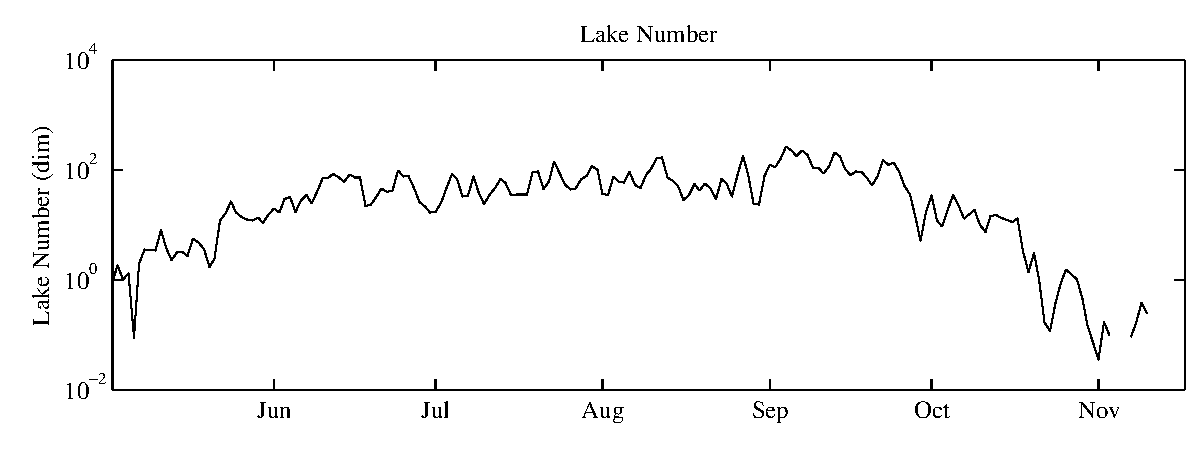
\includegraphics[width = \linewidth]{figures/Sparkling_Ln.pdf}
  \end{subfigure}
  \begin{subfigure}{\lafigsize}
    \caption{\label{fig:la:out:SLn}Seasonal Lake Number}
    \includegraphics[width = \linewidth]{figures/Sparkling_SLn.pdf}
  \end{subfigure}
  \begin{subfigure}{\lafigsize}
    \caption{\label{fig:la:out:metaT}Metalimnion Top}
    \includegraphics[width = \linewidth]{figures/Sparkling_metaT.pdf}
  \end{subfigure}
  \begin{subfigure}{\lafigsize}
    \caption{\label{fig:la:out:metaB}Metalimnion Bottom}
    \includegraphics[width = \linewidth]{figures/Sparkling_metaB.pdf}
  \end{subfigure}
  \begin{subfigure}{\lafigsize}
    \caption{\label{fig:la:out:SmetaT}Seasonal Metalimnion Top}
    \includegraphics[width = \linewidth]{figures/Sparkling_SmetaT.pdf}
  \end{subfigure}
  \begin{subfigure}{\lafigsize}
    \caption{\label{fig:la:out:SmetaB}Seasonal Metalimnion Bottom}
    \includegraphics[width = \linewidth]{figures/Sparkling_SmetaB.pdf}
  \end{subfigure}
  \begin{subfigure}{\lafigsize}
    \caption{\label{fig:la:out:N2}Buoyancy Frequency}
    \includegraphics[width = \linewidth]{figures/Sparkling_N2.pdf}
  \end{subfigure}
  \begin{subfigure}{\lafigsize}
    \caption{\label{fig:la:out:SN2}Seasonal Buoyancy Frequency}
    \includegraphics[width = \linewidth]{figures/Sparkling_SN2.pdf}
  \end{subfigure}
  \begin{subfigure}{\lafigsize}
    \caption{\label{fig:la:out:T1}Mode-1 Vertical Seiche Period}
    \includegraphics[width = \linewidth]{figures/Sparkling_T1.pdf}
  \end{subfigure}
  \begin{subfigure}{\lafigsize}
    \caption{\label{fig:la:out:ST1}Seasonal Mode-1 Vertical Seiche Period}
    \includegraphics[width = \linewidth]{figures/Sparkling_ST1.pdf}
  \end{subfigure}
  \caption[\lafigdesc.]{\label{fig:la:outputs:1}\lafigdesc{} \emph{(continued on \cpageref{fig:la:outputs:2})}.}
\end{figure}
\begin{figure}
  \ContinuedFloat\centering\captionsetup{list=no}
  \begin{subfigure}{\lafigsize}
    \caption{\label{fig:la:out:W}Wedderburn Number}
    \includegraphics[width = \linewidth]{figures/Sparkling_W.pdf}
  \end{subfigure}
  \begin{subfigure}{\lafigsize}
    \caption{\label{fig:la:out:SW}Seasonal Wedderburn Number}
    \includegraphics[width = \linewidth]{figures/Sparkling_SW.pdf}
  \end{subfigure}
  \begin{subfigure}{\lafigsize}
    \caption{\label{fig:la:out:thermD}Thermocline Depth}
    \includegraphics[width = \linewidth]{figures/Sparkling_thermD.pdf}
  \end{subfigure}
  \begin{subfigure}{\lafigsize}
    \caption{\label{fig:la:out:SthermD}Seasonal Thermocline Depth}
    \includegraphics[width = \linewidth]{figures/Sparkling_SthermD.pdf}
  \end{subfigure}
  \begin{subfigure}{\lafigsize}
    \caption{\label{fig:la:out:uSt}$u^{*}$}
    \includegraphics[width = \linewidth]{figures/Sparkling_uSt.pdf}
  \end{subfigure}
  \begin{subfigure}{\lafigsize}
    \caption{\label{fig:la:out:SuSt}Seasonal $u^{*}$}
    \includegraphics[width = \linewidth]{figures/Sparkling_SuSt.pdf}
  \end{subfigure}
  \begin{subfigure}{\lafigsize}
    \caption{\label{fig:la:out:St}Schmidt Stability}
    \includegraphics[width = \linewidth]{figures/Sparkling_St.pdf}
  \end{subfigure}
  \begin{subfigure}{\lafigsize}
    \caption{\label{fig:la:out:wndSpd}Wind Speed}
    \includegraphics[width = \linewidth]{figures/Sparkling_wndSpd.pdf}
  \end{subfigure}
  \begin{subfigure}{\lafigsize}
    \caption{\label{fig:la:out:wTemp}Water Temperature}
    \includegraphics[width = \linewidth]{figures/Sparkling_wTemp.pdf}
  \end{subfigure}
  \caption{\label{fig:la:outputs:2}\lafigdesc.}
\end{figure}


Besides a raw data output as \ac{CSV}, the \la features visualizations of the produced stratification and mixing indices, which can be seen in \cref{fig:la:outputs:1}. Its outputs include Lake Number \citep[see \cref{fig:la:out:Ln,fig:la:out:SLn},][]{imberger1990}, metalimnion extent (see \cref{fig:la:out:metaT,fig:la:out:metaB,fig:la:out:SmetaT,fig:la:out:SmetaB}), Brunt-Väisälä buoyancy frequency (see \cref{fig:la:out:N2,fig:la:out:SN2}), mode-1 vertical seiche period \citep[see \cref{fig:la:out:T1,fig:la:out:ST1},][]{monismith1986}, Wedderburn Number \citep[see \cref{fig:la:out:W,fig:la:out:SW},][]{thompson1980}, thermocline depth (see \cref{fig:la:out:thermD,fig:la:out:SthermD}), $u^{*}$ (wind stress introduced water friction velocity, see \cref{fig:la:out:uSt,fig:la:out:SuSt}) and Schmidt Stability \citep[see \cref{fig:la:out:St},][]{schmidt1928,hutchinson1957,idso1973}. The \la is able to error check and/or down sample input time series and also outputs wind speed (\cref{fig:la:out:wndSpd}) and water temperature (\cref{fig:la:out:wTemp}).

The \la is written as an open source MATLAB application and thus is cross-platform, but requires a MATLAB license and therefore is not easily portable. To overcome this issue, a web portal\footnote{\url{http://lakeanalyzer.gleon.org/} \lastretrievedp} was created that allows the remote \la execution without a local MATLAB installation.

This thesis work comprises the evaluation, design and prototypical implementation of a web-based lake analysis chain for large data sets and live sensor data. Therefore it will evaluate how an analysis language commonly used by domain experts (in this case MATLAB) can easily be deployed in a web-based processing chain, how large scale hydrological data can be processed in a service-based processing chain and whether available web-processing interface definitions support a streaming scenario, or, if not, what is missing to enable streaming processing of geospatial data. Furthermore, this thesis will evaluate how spatial dependencies between streamed features can be modeled and how continuous statistical quality assurance and quality control in the application area of lake ecology can be modeled in a web service chain.

To accomplish this, \cref{sec:wps} features a detailed introduction to the established standard for web-based processing of spatiotemporal data, the OGC \acl{WPS}. In \cref{sec:matlabwps}, a WPS implementation that allows the deployment of generic MATLAB-based software as WPS processes is conceptualized and thus a component to expose the \la using a standardized web processing interface is created. To enable large-scale processing of geospatial data, a Streaming WPS is developed in \cref{sec:streamingwps}, which is not only able to conduct analysis of live hydrological sensor data, but can also be applied to various other use cases. In \cref{sec:conclusion}, the accomplished results are summarized and an outlook about possible future developments and conceivable research topics is given.
